\chapter {Test-driven development}

In the implementation chapter, we mentioned that tests were written during implementation and that the \acrshort{tdd} technique was used.
"Test-driven development is a software development approach in which test cases are developed to specify and validate what the code will do." \cite{hamilton_what_2020}
What this means to us is that before the implementation of any public method, we should write a test for this method.
This chapter will focus on implementing the tests and some base principles of test-driven development and writing tests in general.

We need a framework that will help us write and run tests to write and run tests.
In .NET framework are number of test frameworks that we can use, here is a list of the most used ones:

\begin{itemize}
    \item {MSTest - Microsoft original test framework}
    \item {NUnit - Originaly ported from JUnit \cite{noauthor_nunitorg_nodate}}
    \item {xUnit - Created by author of the NUnit v2 \cite{noauthor_home_nodate}}
\end{itemize}

Per the author's experience, we will use the xUnit framework, but \acrshort{tdd} can be done in any of them.

.NET \acrshort{cli} tool has a template for xUnit project available under command \texttt{dotnet new xunit}. This command will
prepare a project with dependencies for xUnit and Microsoft.NET.Test.Sdk packages. It will also configure runners and coverlet.collector for collecting
code coverage.

\section{More information about \acrshort{tdd}}

Test-driven development can be summed up using an activity diagram.
At the start of the development, we write down all the tests that we need to cover our \acrshort{api}, and then we start with the implementation of the library.
We refactor our code; for example, we move code from one method into multiple methods and even classes.
After refactoring is done, we check our tests and write new ones.

\begin{figure}[H]
    \centering
    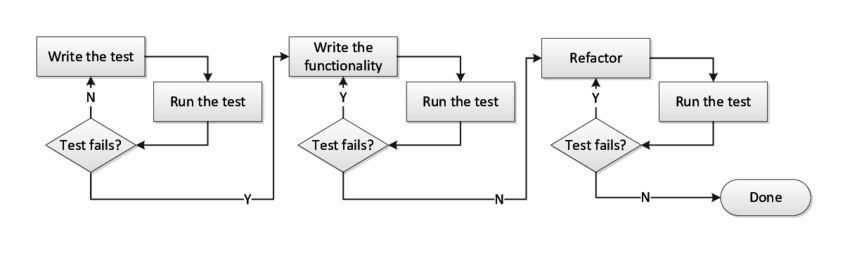
\includegraphics[width=\textwidth]{content/Test-Driven-Development-activities.png}
    \caption{Test-driven development diagram \cite{noauthor_continuous_2013}}
    \label{fig:tddDiagram}
\end{figure}

Using this approach has many benefits. One of them is complete code coverage of our code, which means every method should be covered by a test.
We will use the coverlet tool to calculate the coverage, a cross-platform coverage framework for .NET. \cite{noauthor_coverlet_2022}
It supports multiple output formats, but for our case, we will use \texttt{lcov} format, which can be then loaded by extension in Visual Studio Code and display coverage information directly in files.
We can also generate a report of the coverage using these commands.
\begin{itemize}
    \item {\texttt{dotnet test \textbackslash\\
              /p:CollectCoverage=true \textbackslash\\/p:CoverletOutput=../../lcov.info \textbackslash\\/p:CoverletOutputFormat=lcov}}
    \item {\texttt{genhtml lcov.info -o ./CoverageReport/}}
\end{itemize}
The first command is to execute tests and generate \texttt{lcov.info} file, which contains coverage information. This file is also used by extension for Visual Studio Code
named Coverage Gutters.
The second command is to generate HTML report from \texttt{lcov.info} file.

Figure \ref{fig:report} is an example of the report from this project.

\begin{figure}[H]
    \centering
    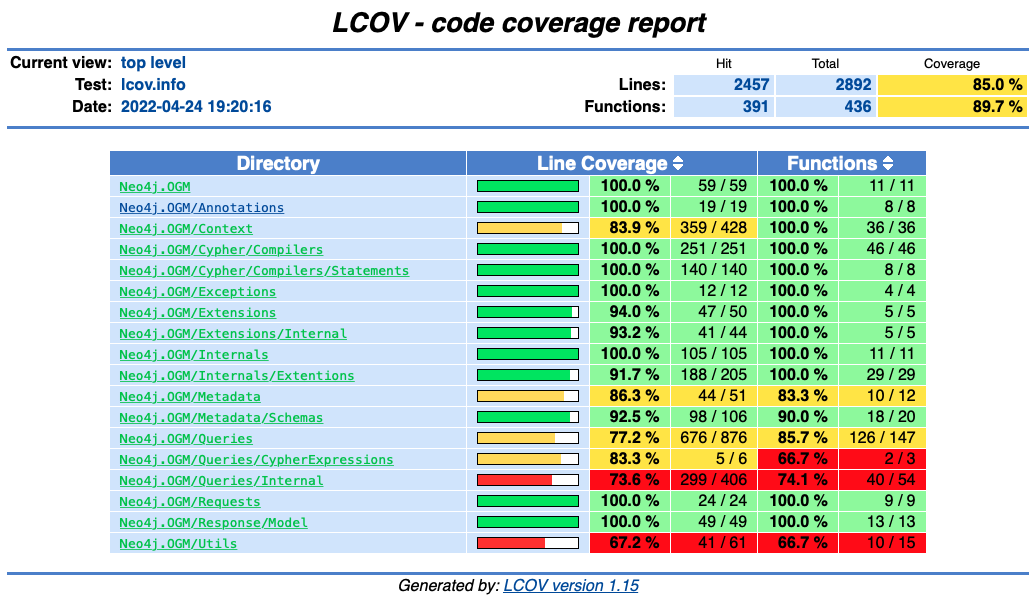
\includegraphics[width=\textwidth]{content/coverage_report.png}
    \caption{Example of the report}
    \label{fig:report}
\end{figure}

We have introduced the concept of \acrshort{tdd} and tools for managing tests.
Now we will go through the process of their implementation.

\section{\texttt{SessionFactory} tests}

We will start with testing \texttt{SessionFactory} as it is the entry point to use our library. Tests will be simple,
we want to test that \texttt{SessionFactory.Create} return an instance of \texttt{ISession} and that if the configuration
set on creating \texttt{SessionFactory} is invalid, that proper exception will be thrown.

\subsection{Mocking}

When writing tests for \texttt{SessionFactory}, we encountered a problem with sending assemblies containing our domain model to the \texttt{SessionFactory} constructor.
We want these assemblies to be mocked.

What is mocking? "Mocking is a process used in unit testing when the unit being tested has external dependencies.
The purpose of mocking is to isolate and focus on the code being tested and not on the behaviour or state of external dependencies.
In mocking, the dependencies are replaced by closely controlled replacements objects that simulate the behaviour of the real ones." \cite{noauthor_mocking_nodate}

For our case, we will use a library for .NET called Moq, which is available as a NuGet package.
More information about this package can be found at \url{https://github.com/moq/moq4}.

The code example \ref{code:SessionFactoryCreateTest} is of one of the tests for \texttt{SessionFactory.Create}, which shows application of mocking.
We mock the \texttt{Assembly} class, and also set up a mocked resuly of the \texttt{Assembly.GetTypes} method.
This method is used internally inside the library, and we need to define our result to be able to inject the suitable array of classes against which we want to run the test.

\begin{listing}[H]
    \begin{minted}[
 frame=lines,
 framesep=2mm,
 baselinestretch=1,
 bgcolor=LightGray,
 linenos,
 breaklines
 ] {csharp}
 public void CreateTestResultOk()
 {
 var assembly = new Moq.Mock<Assembly>();
 assembly.Setup(a => a.GetTypes()).Returns(new[] { typeof(Person), typeof(Post) });

 var sessionFactory = new SessionFactory(
 "connectionString",
 AuthTokens.Basic("username", "password"),
 assembly.Object);

 var session = sessionFactory.Create();

 Assert.NotNull(session);
 Assert.IsAssignableFrom<ISession>(session);
 }
 \end{minted}
    \caption{Example of \texttt{SessionFactory} test with mocking of \texttt{Assembly} object}
    \label{code:SessionFactoryCreateTest}
\end{listing}

\section{Testing internal classes and methods}

In our library, we are using a keyword \texttt{internal} which hides classes, methods, or properties from other assemblies,
but because we also want to test these classes and their methods, we need to expose them. Exposing \texttt{internal} is possible
with a slight change in the project file.
We need to add the code snippet from the code example \ref{code:csprojinternal} to the library project file, and our tests will be able to access every internal class and method.

\begin{listing}[H]
    \begin{minted}[
 frame=lines,
 framesep=2mm,
 baselinestretch=1,
 bgcolor=LightGray,
 linenos,
 breaklines
 ] {xml}
<ItemGroup>
 <AssemblyAttribute
 Include="System.Runtime.CompilerServices.InternalsVisibleTo">
 <_Parameter1>Neo4j.OGM.Tests</_Parameter1>
 </AssemblyAttribute>
</ItemGroup>
 \end{minted}
    \caption{Snippet of \texttt{Neo4j.OGM.csproj} to access internal classes and methods inside test project}
    \label{code:csprojinternal}
\end{listing}

We are using this alteration of the \texttt{Neo4j.OGM.csproj} to access internal classes and methods inside the test project, we can now prepare a test for internal classes and methods.

\section {Setup and cleanup}

Some of our tests will need to prepare data and mocks.
We call this step of tests a setup step.
nUnit for example, uses annotations to mark cleanup (\texttt{TearDownAttribute}) and setup (\texttt{SetUpAttribute}) methods.
However, in xUnit, we are using only constructors, and \texttt{IDisposable} interface for setup and cleanup, respectively.
This approach has a limitation in not being able to perform asynchronous operations safely, but xUnit has a solution for this too.
\texttt{IAsyncLifetime} is an interface from xUnit that provides the means to perform setup and cleanup methods asynchronously.

Apart from setup and cleanup methods, xUnit also offers an ability to share context between tests, either in one class or across multiple classes using class fixtures or collection fixtures. More on this subject can be found in the official documentation of the xUnit framework. \cite{noauthor_home_nodate}

\section {Summary}

We have now described all the parts of our testing, tests are ready, and we can start with the cycle of implementation and testing as described in \acrshort{tdd} diagram in the figure \ref{fig:tddDiagram}.
This chapter was put after the implementation for clarity reasons.